% =========================================================================
% BÀI 19: ÔN TẬP HÌNH HỌC (HÌNH PHẲNG VÀ HÌNH KHỐI - TOÁN LỚP 1)
% TOÀN BỘ CÂU HỎI ĐƯỢC VẼ HÌNH MINH HỌA TRỰC QUAN 100% BẰNG TIKZ 2D & 3D
% =========================================================================

% --- CÁC HÀM VẼ KHỐI 3D VÀ QUE TÍNH CHO BÀI 19 ---

\providecommand{\VeKhoiLapPhuong}[4][yellow!60]{% #1=màu, #2=x, #3=y, #4=cạnh
  \begin{scope}[shift={(#2,#3)}]
    \pgfmathsetmacro{\s}{#4}
    \pgfmathsetmacro{\dx}{\s*0.42}
    \pgfmathsetmacro{\dy}{\s*0.32}
    \draw[fill=#1, draw=black!75, line width=1.1pt] (0,0) rectangle (\s,\s);
    \draw[fill=white!35!#1, draw=black!75, line width=1.1pt] (0,\s) -- (\s,\s) -- (\s+\dx,\s+\dy) -- (\dx,\s+\dy) -- cycle;
    \draw[fill=black!25!#1, draw=black!75, line width=1.1pt] (\s,0) -- (\s+\dx,\dy) -- (\s+\dx,\s+\dy) -- (\s,\s) -- cycle;
  \end{scope}
}

\providecommand{\VeKhoiHopChuNhat}[6][cyan!50]{% #1=màu, #2=x, #3=y, #4=rộng, #5=cao, #6=sâu
  \begin{scope}[shift={(#2,#3)}]
    \pgfmathsetmacro{\w}{#4}
    \pgfmathsetmacro{\h}{#5}
    \pgfmathsetmacro{\dx}{#6*0.42}
    \pgfmathsetmacro{\dy}{#6*0.32}
    \draw[fill=#1, draw=black!75, line width=1.1pt] (0,0) rectangle (\w,\h);
    \draw[fill=white!35!#1, draw=black!75, line width=1.1pt] (0,\h) -- (\w,\h) -- (\w+\dx,\h+\dy) -- (\dx,\h+\dy) -- cycle;
    \draw[fill=black!25!#1, draw=black!75, line width=1.1pt] (\w,0) -- (\w+\dx,\dy) -- (\w+\dx,\h+\dy) -- (\w,\h) -- cycle;
  \end{scope}
}

\providecommand{\VeQueTinh}[4]{% #1=x1, #2=y1, #3=x2, #4=y2
  \draw[line width=3pt, orange!80!yellow, line cap=round] (#1,#2) -- (#3,#4);
  \fill[red!90!black] (#1,#2) circle (0.08cm);
}

% =========================================================================
% PHẦN 1: TRẮC NGHIỆM LỰA CHỌN (12 CÂU) - ĐÁP ÁN ĐƯỢC PHÂN BỔ ĐỀU A, B, C, D
% =========================================================================
\textbf{Phần 1. Trắc nghiệm lựa chọn}
\setcounterpageref{ex}{0}

% --- CÂU 1 ---
\begin{ex} %[1H5N19]
Trong các hình dưới đây, hình nào có đúng $3$ cạnh và $3$ đỉnh?
\begin{center}
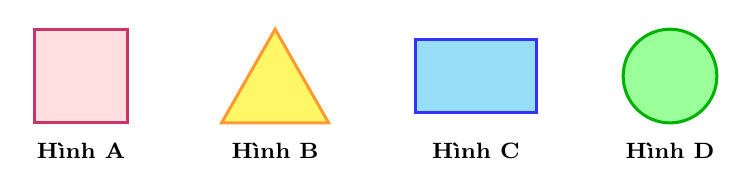
\begin{tikzpicture}[scale=0.85, baseline=(current bounding box.center)]
  % Hình vuông
  \begin{scope}[shift={(0,0)}]
    \draw[fill=pink!50, draw=purple!80, line width=1.1pt] (0,0) rectangle (1.4,1.4);
    \node[below, font=\bfseries\footnotesize] at (0.7,-0.15) {Hình A};
  \end{scope}
  % Hình tam giác
  \begin{scope}[shift={(2.8,0)}]
    \draw[fill=yellow!60, draw=orange!80, line width=1.1pt] (0,0) -- (1.6,0) -- (0.8,1.4) -- cycle;
    \node[below, font=\bfseries\footnotesize] at (0.8,-0.15) {Hình B};
  \end{scope}
  % Hình chữ nhật
  \begin{scope}[shift={(5.7,0)}]
    \draw[fill=cyan!40, draw=blue!80, line width=1.1pt] (0,0.15) rectangle (1.8,1.25);
    \node[below, font=\bfseries\footnotesize] at (0.9,-0.15) {Hình C};
  \end{scope}
  % Hình tròn
  \begin{scope}[shift={(8.8,0)}]
    \draw[fill=green!40, draw=green!70!black, line width=1.1pt] (0.7,0.7) circle (0.7cm);
    \node[below, font=\bfseries\footnotesize] at (0.7,-0.15) {Hình D};
  \end{scope}
\end{tikzpicture}
\end{center}
\choice
{\True Hình B (Hình tam giác)}
{Hình A (Hình vuông)}
{Hình C (Hình chữ nhật)}
{Hình D (Hình tròn)}
\loigiai{
Hình tam giác (Hình B) có đúng $3$ cạnh và $3$ đỉnh.\\
\textbf{Đáp án của câu hỏi là A}
}
\end{ex}

% --- CÂU 2 ---
\begin{ex} %[1H5N19]
Hình nào dưới đây là hình vuông (có $4$ cạnh dài bằng nhau)?
\begin{center}
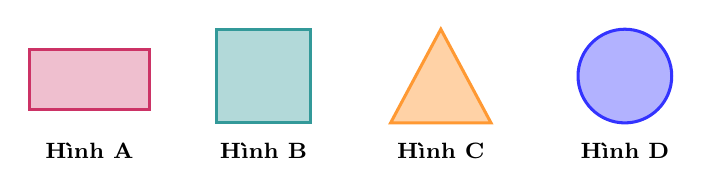
\begin{tikzpicture}[scale=0.85, baseline=(current bounding box.center)]
  % A: Hình chữ nhật
  \begin{scope}[shift={(0,0)}]
    \draw[fill=purple!25, draw=purple!80, line width=1.1pt] (0,0.2) rectangle (1.8,1.1);
    \node[below, font=\bfseries\footnotesize] at (0.9,-0.15) {Hình A};
  \end{scope}
  % B: Hình vuông
  \begin{scope}[shift={(2.8,0)}]
    \draw[fill=teal!30, draw=teal!80, line width=1.1pt] (0,0) rectangle (1.4,1.4);
    \node[below, font=\bfseries\footnotesize] at (0.7,-0.15) {Hình B};
  \end{scope}
  % C: Hình tam giác
  \begin{scope}[shift={(5.4,0)}]
    \draw[fill=orange!35, draw=orange!80, line width=1.1pt] (0,0) -- (1.5,0) -- (0.75,1.4) -- cycle;
    \node[below, font=\bfseries\footnotesize] at (0.75,-0.15) {Hình C};
  \end{scope}
  % D: Hình tròn
  \begin{scope}[shift={(8.2,0)}]
    \draw[fill=blue!30, draw=blue!80, line width=1.1pt] (0.7,0.7) circle (0.7cm);
    \node[below, font=\bfseries\footnotesize] at (0.7,-0.15) {Hình D};
  \end{scope}
\end{tikzpicture}
\end{center}
\choice
{\True Hình B}
{Hình A}
{Hình C}
{Hình D}
\loigiai{
Hình B có $4$ cạnh bằng nhau là hình vuông.\\
\textbf{Đáp án của câu hỏi là A}
}
\end{ex}

% --- CÂU 3 ---
\begin{ex} %[1H5H19]
Bao diêm dưới đây có dạng hình khối nào mà em đã học?
\begin{center}
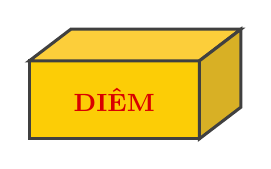
\begin{tikzpicture}[scale=0.9, baseline=(current bounding box.center)]
  \VeKhoiHopChuNhat[yellow!65!orange]{0}{0}{2.4}{1.1}{1.4}
  \node[font=\bfseries\small, text=red!85!black] at (1.2,0.55) {DIÊM};
\end{tikzpicture}
\end{center}
\choice
{Khối lập phương}
{Hình chữ nhật}
{\True Khối hộp chữ nhật}
{Hình tam giác}
\loigiai{
Bao diêm là một khối hộp chữ nhật trong không gian 3 chiều.\\
\textbf{Đáp án của câu hỏi là C}
}
\end{ex}

% --- CÂU 4 ---
\begin{ex} %[1H5H19]
Viên xúc xắc đồ chơi dưới đây có dạng hình khối gì?
\begin{center}
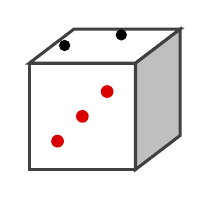
\begin{tikzpicture}[scale=0.9, baseline=(current bounding box.center)]
  \VeKhoiLapPhuong[white]{0}{0}{1.5}
  % Chấm tròn xúc xắc mặt trước: số 3
  \fill[red!85!black] (0.4,0.4) circle (0.09cm);
  \fill[red!85!black] (0.75,0.75) circle (0.09cm);
  \fill[red!85!black] (1.1,1.1) circle (0.09cm);
  % Mặt trên: số 2
  \fill[black] (0.5,1.75) circle (0.08cm);
  \fill[black] (1.3,1.9) circle (0.08cm);
\end{tikzpicture}
\end{center}
\choice
{Khối hộp chữ nhật}
{Hình vuông}
{Khối cầu}
{\True Khối lập phương}
\loigiai{
Viên xúc xắc có $6$ mặt đều là hình vuông bằng nhau nên có dạng khối lập phương.\\
\textbf{Đáp án của câu hỏi là D}
}
\end{ex}

\newpage

% --- CÂU 5 ---
\begin{ex} %[1H5H19]
Khối lập phương có tất cả bao nhiêu mặt phẳng bao quanh?
\begin{center}
\begin{tikzpicture}[scale=0.85, baseline=(current bounding box.center)]
  \VeKhoiLapPhuong[cyan!40]{0}{0}{1.4}
  \node[right, font=\bfseries\footnotesize, text=blue!85!black] at (2.4,0.7) {Gồm mặt trên, dưới, trước, sau, trái, phải};
\end{tikzpicture}
\end{center}
\choice
{\True $6$ mặt vuông bằng nhau}
{$4$ mặt}
{$8$ mặt}
{$5$ mặt}
\loigiai{
Khối lập phương có đúng $6$ mặt và tất cả đều là các hình vuông bằng nhau.\\
\textbf{Đáp án của câu hỏi là A}
}
\end{ex}

% --- CÂU 6 ---
\begin{ex} %[1H5H19]
Hình nào sau đây được tạo bởi một đường cong khép kín, không có cạnh thẳng và không có góc?
\begin{center}
\begin{tikzpicture}[scale=0.85, baseline=(current bounding box.center)]
  \begin{scope}[shift={(0,0)}]
    \draw[fill=orange!35, draw=orange!80, line width=1.1pt] (0,0) -- (1.5,0) -- (0.75,1.3) -- cycle;
    \node[below, font=\bfseries\footnotesize] at (0.75,-0.1) {Tam giác};
  \end{scope}
  \begin{scope}[shift={(3.0,0)}]
    \draw[fill=yellow!60, draw=red!70, line width=1.2pt] (0.7,0.7) circle (0.7cm);
    \node[below, font=\bfseries\footnotesize] at (0.7,-0.1) {Hình tròn};
  \end{scope}
  \begin{scope}[shift={(5.8,0)}]
    \draw[fill=teal!30, draw=teal!80, line width=1.1pt] (0,0) rectangle (1.3,1.3);
    \node[below, font=\bfseries\footnotesize] at (0.65,-0.1) {Hình vuông};
  \end{scope}
  \begin{scope}[shift={(8.4,0)}]
    \draw[fill=blue!25, draw=blue!80, line width=1.1pt] (0,0.15) rectangle (1.6,1.15);
    \node[below, font=\bfseries\footnotesize] at (0.8,-0.1) {Chữ nhật};
  \end{scope}
\end{tikzpicture}
\end{center}
\choice
{Hình tam giác}
{\True Hình tròn}
{Hình vuông}
{Hình chữ nhật}
\loigiai{
Hình tròn là hình phẳng được bao quanh bởi đường cong tròn khép kín, không có cạnh thẳng và không có đỉnh/góc.\\
\textbf{Đáp án của câu hỏi là B}
}
\end{ex}

% --- CÂU 7 ---
\begin{ex} %[1H5V19]
Để ghép thành một khung hình vuông như hình dưới đây, em cần dùng bao nhiêu que tính có độ dài bằng nhau?
\begin{center}
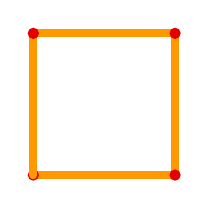
\begin{tikzpicture}[scale=0.9, baseline=(current bounding box.center)]
  \VeQueTinh{0}{0}{2}{0}
  \VeQueTinh{2}{0}{2}{2}
  \VeQueTinh{2}{2}{0}{2}
  \VeQueTinh{0}{2}{0}{0}
\end{tikzpicture}
\end{center}
\choice
{$3$ que tính}
{$5$ que tính}
{\True $4$ que tính}
{$6$ que tính}
\loigiai{
Hình vuông có $4$ cạnh bằng nhau nên cần đúng $4$ que tính để ghép.\\
\textbf{Đáp án của câu hỏi là C}
}
\end{ex}

% --- CÂU 8 ---
\begin{ex} %[1H5V19]
Để ghép được $2$ hình tam giác riêng biệt như hình dưới, cần tất cả bao nhiêu que tính?
\begin{center}
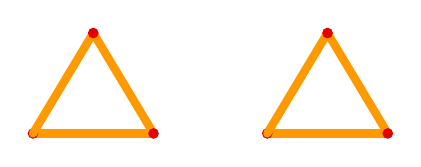
\begin{tikzpicture}[scale=0.85, baseline=(current bounding box.center)]
  % Tam giác 1
  \VeQueTinh{0}{0}{1.8}{0}
  \VeQueTinh{1.8}{0}{0.9}{1.5}
  \VeQueTinh{0.9}{1.5}{0}{0}
  % Tam giác 2
  \begin{scope}[shift={(3.5,0)}]
    \VeQueTinh{0}{0}{1.8}{0}
    \VeQueTinh{1.8}{0}{0.9}{1.5}
    \VeQueTinh{0.9}{1.5}{0}{0}
  \end{scope}
\end{tikzpicture}
\end{center}
\choice
{$5$ que tính}
{\True $6$ que tính}
{$7$ que tính}
{$4$ que tính}
\loigiai{
Mỗi hình tam giác cần $3$ que tính. Hai hình tam giác riêng biệt cần: $3 + 3 = 6$ que tính.\\
\textbf{Đáp án của câu hỏi là B}
}
\end{ex}

\newpage

% --- CÂU 9 ---
\begin{ex} %[1H5V19]
Hình con thuyền dưới đây được ghép bởi bao nhiêu hình tam giác?
\begin{center}
\begin{tikzpicture}[scale=0.85, baseline=(current bounding box.center)]
  % Cánh buồm (2 tam giác)
  \draw[fill=yellow!70, draw=orange!90!black, line width=1.1pt] (2,1.2) -- (2,3.2) -- (0.8,1.2) -- cycle;
  \draw[fill=red!70, draw=red!90!black, line width=1.1pt] (2.1,1.2) -- (2.1,3.4) -- (3.6,1.2) -- cycle;
  % Cột buồm
  \draw[line width=2pt, brown!80!black] (2.05,0.8) -- (2.05,3.5);
  % Thân thuyền (hình thang ghép từ 3 tam giác hoặc đáy thuyền)
  \draw[fill=cyan!40, draw=blue!80, line width=1.1pt] (0,0.8) -- (0.8,0) -- (3.4,0) -- (4.2,0.8) -- cycle;
  \draw[line width=1pt, blue!80, dashed] (0.8,0) -- (0.8,0.8);
  \draw[line width=1pt, blue!80, dashed] (3.4,0) -- (3.4,0.8);
  \node[font=\footnotesize\itshape, text=blue!80!black] at (2.1,-0.4) {(Cánh buồm gồm 2 hình tam giác)};
\end{tikzpicture}
\end{center}
\choice
{$1$ hình tam giác}
{$3$ hình tam giác}
{$4$ hình tam giác}
{\True $2$ hình tam giác ở cánh buồm}
\loigiai{
Hai cánh buồm của con thuyền là $2$ hình tam giác.\\
\textbf{Đáp án của câu hỏi là D}
}
\end{ex}

% --- CÂU 10 ---
\begin{ex} %[1H5V19]
Quan sát chú robot bằng gỗ dưới đây. Chú robot được tạo thành từ bao nhiêu khối lập phương màu vàng?
\begin{center}
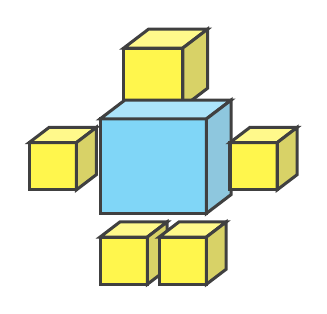
\begin{tikzpicture}[scale=0.75, baseline=(current bounding box.center)]
  % Đầu: 1 khối lập phương
  \VeKhoiLapPhuong[yellow!70]{1.4}{3.2}{1.0}
  % Thân: 1 khối hộp chữ nhật
  \VeKhoiHopChuNhat[cyan!50]{1.0}{1.4}{1.8}{1.6}{1.0}
  % Hai tay: 2 khối lập phương
  \VeKhoiLapPhuong[yellow!70]{-0.2}{1.8}{0.8}
  \VeKhoiLapPhuong[yellow!70]{3.2}{1.8}{0.8}
  % Hai chân: 2 khối lập phương
  \VeKhoiLapPhuong[yellow!70]{1.0}{0.2}{0.8}
  \VeKhoiLapPhuong[yellow!70]{2.0}{0.2}{0.8}
\end{tikzpicture}
\end{center}
\choice
{$4$ khối}
{$6$ khối}
{\True $5$ khối lập phương màu vàng}
{$3$ khối}
\loigiai{
Đếm các khối lập phương màu vàng: 1 khối làm đầu, 2 khối làm tay, 2 khối làm chân. Tổng cộng có: $1 + 2 + 2 = 5$ khối lập phương.\\
\textbf{Đáp án của câu hỏi là C}
}
\end{ex}

% --- CÂU 11 ---
\begin{ex} %[1H5V19]
Quan sát bức tranh: Quả bóng màu đỏ đang ở vị trí nào so với chiếc bàn học?
\begin{center}
\begin{tikzpicture}[scale=0.85, baseline=(current bounding box.center)]
  % Bàn học
  \draw[fill=brown!50, draw=brown!80!black, line width=1.2pt] (0,1.2) rectangle (4,1.5);
  \draw[fill=brown!70!black] (0.3,0) rectangle (0.6,1.2);
  \draw[fill=brown!70!black] (3.4,0) rectangle (3.7,1.2);
  % Quyển vở trên bàn
  \draw[fill=blue!30, draw=blue!80] (1.2,1.5) rectangle (2.2,1.75);
  % Quả bóng dưới gầm bàn
  \shadedraw[ball color=red, draw=black!70] (2,0.4) circle (0.35cm);
  \node[font=\bfseries\footnotesize, text=red!80!black] at (2,-0.4) {Quả bóng};
\end{tikzpicture}
\end{center}
\choice
{Ở trên mặt bàn}
{\True Ở dưới gầm bàn}
{Ở bên phải cái bàn}
{Ở bên trái cái bàn}
\loigiai{
Quả bóng màu đỏ nằm ở vị trí phía dưới (dưới gầm) chiếc bàn.\\
\textbf{Đáp án của câu hỏi là B}
}
\end{ex}

% --- CÂU 12 ---
\begin{ex} %[1H5V19]
Trong các đồ vật sau, đồ vật nào có dạng \textbf{hình tròn}?
\begin{center}
\begin{tikzpicture}[scale=0.85, baseline=(current bounding box.center)]
  % Thước kẻ hình chữ nhật
  \begin{scope}[shift={(0,0)}]
    \draw[fill=yellow!30, draw=orange!80, line width=1pt] (0,0.2) rectangle (2.0,0.9);
    \node[below, font=\bfseries\footnotesize] at (1.0,-0.1) {Thước kẻ};
  \end{scope}
  % Mặt đồng hồ hình tròn
  \begin{scope}[shift={(3.0,0)}]
    \draw[fill=cyan!20, draw=blue!80, line width=1.2pt] (0.7,0.7) circle (0.65cm);
    \draw[line width=1pt] (0.7,0.7) -- (0.7,1.1);
    \draw[line width=1.2pt] (0.7,0.7) -- (1.0,0.7);
    \node[below, font=\bfseries\footnotesize] at (0.7,-0.1) {Đồng hồ};
  \end{scope}
  % Khung ảnh vuông
  \begin{scope}[shift={(5.8,0)}]
    \draw[fill=pink!30, draw=purple!80, line width=1pt] (0,0) rectangle (1.3,1.3);
    \node[below, font=\bfseries\footnotesize] at (0.65,-0.1) {Khung ảnh};
  \end{scope}
  % Hộp quà khối lập phương
  \begin{scope}[shift={(8.6,0)}]
    \VeKhoiLapPhuong[green!40]{0}{0.1}{1.1}
    \node[below, font=\bfseries\footnotesize] at (0.6,-0.1) {Hộp quà};
  \end{scope}
\end{tikzpicture}
\end{center}
\choice
{Cái thước kẻ}
{Khung ảnh}
{Hộp quà}
{\True Mặt chiếc đồng hồ treo tường}
\loigiai{
Mặt chiếc đồng hồ treo tường có dạng hình tròn.\\
\textbf{Đáp án của câu hỏi là D}
}
\end{ex}

\newpage

% =========================================================================
% PHẦN 2: CÂU ĐÚNG / SAI (2 CÂU, MỖI CÂU 4 Ý)
% =========================================================================
\textbf{Phần 2. Câu trắc nghiệm đúng sai}
\setcounterpageref{ex}{0}

% --- CÂU 13 ---
\begin{ex} %[1H5H19]
Quan sát ngôi nhà tí hon được ghép từ các khối hình học dưới đây:
\begin{center}
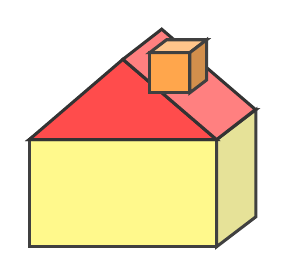
\begin{tikzpicture}[scale=0.85, baseline=(current bounding box.center)]
  % Khối hộp chữ nhật lớn làm thân nhà
  \VeKhoiHopChuNhat[yellow!45]{0}{0}{2.8}{1.6}{1.4}
  % Mái nhà dạng lăng trụ tam giác / khối
  \draw[fill=red!70, draw=black!80, line width=1.1pt] (0,1.6) -- (1.4,2.8) -- (2.8,1.6) -- cycle;
  \draw[fill=red!50!white, draw=black!80, line width=1.1pt] (1.4,2.8) -- (1.4+0.58,2.8+0.45) -- (2.8+0.58,1.6+0.45) -- (2.8,1.6) -- cycle;
  % Ống khói là khối lập phương
  \VeKhoiLapPhuong[orange!70]{1.8}{2.3}{0.6}
\end{tikzpicture}
\end{center}
Xét tính Đúng hay Sai của các khẳng định sau:
\choiceTF
{\True Thân ngôi nhà có dạng khối hộp chữ nhật}
{Ống khói của ngôi nhà có dạng khối cầu}
{\True Mặt trước của thân nhà có dạng hình chữ nhật}
{Ngôi nhà có đúng $5$ khối lập phương}
\loigiai{
a) Thân nhà là khối hộp chữ nhật $\to$ \textbf{Đúng}.\\
b) Ống khói có dạng khối lập phương, không phải khối cầu $\to$ \textbf{Sai}.\\
c) Mặt trước thân nhà là một hình chữ nhật phẳng $\to$ \textbf{Đúng}.\\
d) Chỉ có $1$ khối lập phương làm ống khói (không phải 5) $\to$ \textbf{Sai}.
}
\end{ex}

% --- CÂU 14 ---
\begin{ex} %[1H5V19]
Bức tranh phong cảnh quê hương của bạn Mai được ghép từ các hình phẳng:
\begin{center}
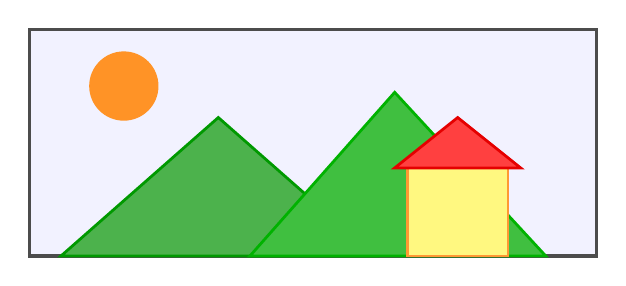
\begin{tikzpicture}[scale=0.8, baseline=(current bounding box.center)]
  % Khung tranh
  \draw[draw=black!70, fill=blue!5, line width=1.2pt] (0,0) rectangle (9.0,3.6);
  % Mặt trời: 1 hình tròn
  \fill[orange!85] (1.5,2.7) circle (0.55cm);
  % Hai ngọn núi: 2 hình tam giác
  \draw[fill=green!40!gray, draw=green!60!black, line width=1pt] (0.5,0) -- (3.0,2.2) -- (5.5,0) -- cycle;
  \draw[fill=green!50!gray, draw=green!70!black, line width=1pt] (3.5,0) -- (5.8,2.6) -- (8.2,0) -- cycle;
  % Thân nhà: 1 hình vuông
  \draw[fill=yellow!50, draw=orange!80, line width=1pt] (6.0,0) rectangle (7.6,1.4);
  % Mái nhà: 1 hình tam giác
  \draw[fill=red!75, draw=red!90!black, line width=1pt] (5.8,1.4) -- (6.8,2.2) -- (7.8,1.4) -- cycle;
\end{tikzpicture}
\end{center}
Xét tính Đúng hay Sai của các khẳng định sau:
\choiceTF
{\True Mặt trời trong bức tranh có dạng hình tròn}
{Bức tranh có tất cả 5 hình tam giác}
{\True Mái nhà và các ngọn núi đều có dạng hình tam giác}
{Thân ngôi nhà có dạng hình tròn}
\loigiai{
a) Mặt trời là hình tròn $\to$ \textbf{Đúng}.\\
b) Có $2$ ngọn núi tam giác và $1$ mái nhà tam giác, tổng cộng $3$ hình tam giác (chứ không phải 5) $\to$ \textbf{Sai}.\\
c) Mái nhà và ngọn núi đều là hình tam giác $\to$ \textbf{Đúng}.\\
d) Thân nhà là hình vuông/chữ nhật, không phải hình tròn $\to$ \textbf{Sai}.
}
\end{ex}

\newpage

% =========================================================================
% PHẦN 3: CÂU TRẢ LỜI NGẮN (6 CÂU)
% =========================================================================
\textbf{Phần 3. Câu trắc nghiệm trả lời ngắn}
\setcounterpageref{ex}{0}

% --- CÂU 15 ---
\begin{ex} %[1H5H19]
Hình vẽ dưới đây có bao nhiêu hình tam giác nhỏ màu xanh?
\begin{center}
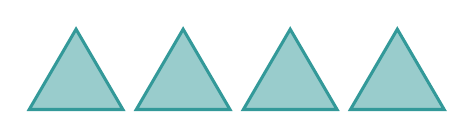
\begin{tikzpicture}[scale=0.85, baseline=(current bounding box.center)]
  \foreach \x in {0, 1.6, 3.2, 4.8}{
    \draw[fill=teal!40, draw=teal!80, line width=1.1pt] (\x,0) -- (\x+1.4,0) -- (\x+0.7,1.2) -- cycle;
  }
\end{tikzpicture}
\end{center}
\textbf{Trả lời:} \raisebox{-2pt}{\framebox[1.5cm]{\phantom{1}}}
\loigiai{
Đếm số hình tam giác: có $4$ hình tam giác.\\
\textbf{Đáp số:} 4
}
\end{ex}

% --- CÂU 16 ---
\begin{ex} %[1H5H19]
Quan sát chồng tháp xếp hình dưới đây. Hỏi có bao nhiêu khối lập phương màu vàng?
\begin{center}
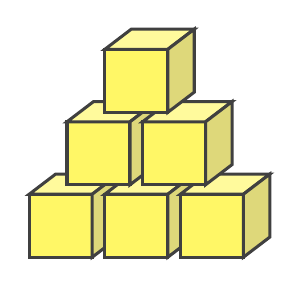
\begin{tikzpicture}[scale=0.8, baseline=(current bounding box.center)]
  % Tầng 1 (đáy): 3 khối
  \VeKhoiLapPhuong[yellow!60]{0}{0}{1.0}
  \VeKhoiLapPhuong[yellow!60]{1.2}{0}{1.0}
  \VeKhoiLapPhuong[yellow!60]{2.4}{0}{1.0}
  % Tầng 2: 2 khối
  \VeKhoiLapPhuong[yellow!60]{0.6}{1.15}{1.0}
  \VeKhoiLapPhuong[yellow!60]{1.8}{1.15}{1.0}
  % Tầng 3 (đỉnh): 1 khối
  \VeKhoiLapPhuong[yellow!60]{1.2}{2.3}{1.0}
\end{tikzpicture}
\end{center}
\textbf{Trả lời:} \raisebox{-2pt}{\framebox[1.5cm]{\phantom{1}}}
\loigiai{
Tầng đáy có $3$ khối, tầng hai có $2$ khối, tầng trên cùng có $1$ khối. Tổng cộng có: $3 + 2 + 1 = 6$ khối lập phương.\\
\textbf{Đáp số:} 6
}
\end{ex}

% --- CÂU 17 ---
\begin{ex} %[1H5V19]
Em cần dùng bao nhiêu que tính để xếp thành một hình chữ nhật như hình dưới?
\begin{center}
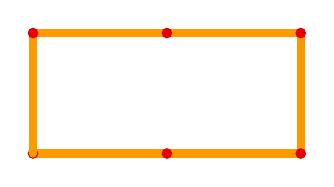
\begin{tikzpicture}[scale=0.85, baseline=(current bounding box.center)]
  % Chiều dài gồm 2 que mỗi bên, chiều rộng 1 que mỗi bên
  \VeQueTinh{0}{0}{2}{0} \VeQueTinh{2}{0}{4}{0}
  \VeQueTinh{4}{0}{4}{1.8}
  \VeQueTinh{4}{1.8}{2}{1.8} \VeQueTinh{2}{1.8}{0}{1.8}
  \VeQueTinh{0}{1.8}{0}{0}
\end{tikzpicture}
\end{center}
\textbf{Trả lời:} \raisebox{-2pt}{\framebox[1.5cm]{\phantom{1}}}
\loigiai{
Mỗi chiều dài gồm $2$ que tính, mỗi chiều rộng gồm $1$ que tính. Tổng số que tính là: $2 + 2 + 1 + 1 = 6$ que tính.\\
\textbf{Đáp số:} 6
}
\end{ex}

% --- CÂU 18 ---
\begin{ex} %[1H5V19]
Hình lớn dưới đây được chia đôi bởi một đường thẳng kẻ dọc. Hỏi có tất cả bao nhiêu hình tam giác trong hình vẽ?
\begin{center}
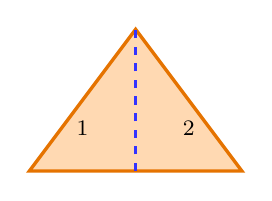
\begin{tikzpicture}[scale=0.9, baseline=(current bounding box.center)]
  \draw[fill=orange!30, draw=orange!90!black, line width=1.2pt] (0,0) -- (3,0) -- (1.5,2) -- cycle;
  \draw[line width=1.2pt, blue!80, dashed] (1.5,0) -- (1.5,2);
  \node[font=\footnotesize] at (0.75,0.6) {1};
  \node[font=\footnotesize] at (2.25,0.6) {2};
\end{tikzpicture}
\end{center}
\textbf{Trả lời:} \raisebox{-2pt}{\framebox[1.5cm]{\phantom{1}}}
\loigiai{
Có $2$ hình tam giác nhỏ và $1$ hình tam giác lớn bao ngoài. Tổng cộng có: $2 + 1 = 3$ hình tam giác.\\
\textbf{Đáp số:} 3
}
\end{ex}

% --- CÂU 19 ---
\begin{ex} %[1H5V19]
Một hình vuông lớn được chia thành các ô vuông nhỏ như bàn cờ. Hỏi hình dưới đây có bao nhiêu hình vuông nhỏ?
\begin{center}
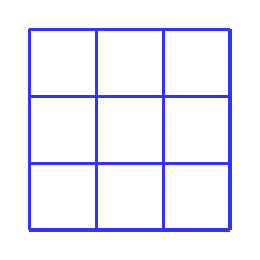
\begin{tikzpicture}[scale=0.85, baseline=(current bounding box.center)]
  \draw[fill=cyan!15, draw=blue!80, line width=1.2pt] (0,0) grid[step=1cm] (3,3);
\end{tikzpicture}
\end{center}
\textbf{Trả lời:} \raisebox{-2pt}{\framebox[1.5cm]{\phantom{1}}}
\loigiai{
Đếm số ô vuông đơn kích thước $1 \times 1$: có $3 \times 3 = 9$ hình vuông nhỏ.\\
\textbf{Đáp số:} 9
}
\end{ex}

% --- CÂU 20 ---
\begin{ex} %[1H5V19]
Quan sát đoàn tàu chở các khối hộp chữ nhật dưới đây. Hỏi đoàn tàu chở tất cả bao nhiêu khối hộp chữ nhật?
\begin{center}
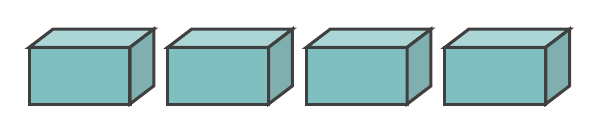
\begin{tikzpicture}[scale=0.8, baseline=(current bounding box.center)]
  \foreach \i in {0,...,3}{
    \VeKhoiHopChuNhat[teal!50]{\i*2.2}{0}{1.6}{0.9}{0.9}
  }
\end{tikzpicture}
\end{center}
\textbf{Trả lời:} \raisebox{-2pt}{\framebox[1.5cm]{\phantom{1}}}
\loigiai{
Đếm số khối hộp chữ nhật: có $4$ khối.\\
\textbf{Đáp số:} 4
}
\end{ex}
